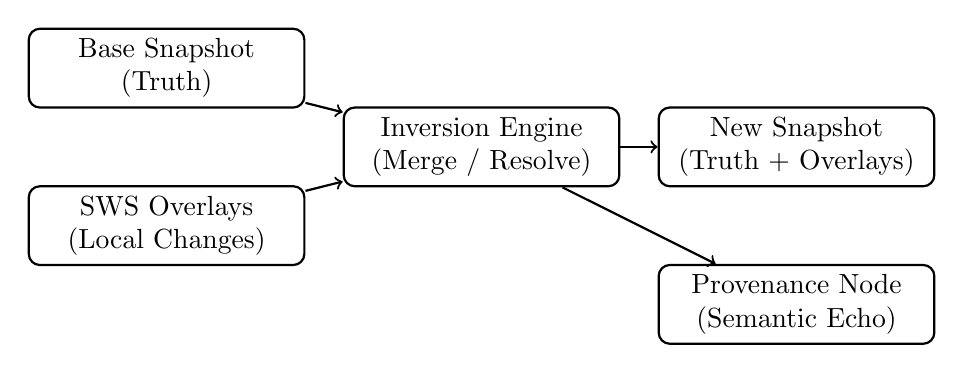
\begin{tikzpicture}[
    process/.style={rectangle, draw=black, thick, rounded corners, minimum width=3.5cm, minimum height=1cm, align=center},
    arrow/.style={->, thick}
]

\node[process] (base)   at (0,0)   {Base Snapshot\\(Truth)};
\node[process] (overlay) at (0,-2) {SWS Overlays\\(Local Changes)};
\node[process] (merge)  at (4,-1)  {Inversion Engine\\(Merge / Resolve)};
\node[process] (snap)   at (8,-1)  {New Snapshot\\(Truth + Overlays)};
\node[process] (prov)   at (8,-3)  {Provenance Node\\(Semantic Echo)};

\draw[arrow] (base) -- (merge);
\draw[arrow] (overlay) -- (merge);
\draw[arrow] (merge) -- (snap);
\draw[arrow] (merge) -- (prov);

\end{tikzpicture}